%%%%%%%%%%%%%%%%%%%%%%%%%%%%%%%%%%%%%%%%%%%%%%%
%%%%%%%%%%%%%%%%%%%%%%%%%%%%%%%
\documentclass{l3deliverable}
%%%%%%%%%%%%%%%%%%%%%%%%%%%%%%%%%%%%%%%%%%%%%%%
%%%%%%%%%%%%%%%%%%%%%%%%%%%%%%%
\usepackage{graphicx}%
\usepackage{tabularx}%
\usepackage{url}%
\usepackage{usecasedescription}%
%%%%%%%%%%%%%%%%%%%%%%%%%%%%%%%%%%%%%%%%%%%%%%%
%%%%%%%%%%%%%%%%%%%%%%%%%%%%%%%
%% Check these macro values for appropriateness for your own document.
\title{Requirements Document}
\author{Ross Adam\\
Andrew Gardner\\
Nicole Kearns\\
Mamas Nicolaou\\
Asset Sarsengaliyev\\
}
\date{1st November 2012}
\deliverableID{D3}
\project{PSD3 Group Exercise 1}
\team{V}
\version{1.5}
%%%%%%%%%%%%%%%%%%%%%%%%%%%%%%%%%%%%%%%%%%%%%%%
%%%%%%%%%%%%%%%%%%%%%%%%%%%%%%%
\begin{document}
%%%%%%%%%%%%%%%%%%%%%%%%%%%%%%%%%%%%%%%%%%%%%%%
%%%%%%%%%%%%%%%%%%%%%%%%%%%%%%%
\maketitle
\tableofcontents
\newpage
%%%%%%%%%%%%%%%%%%%%%%%%%%%%%%%%%%%%%%%%%%%%%%%
%%%%%%%%%%%%%%%%%%%%%%%%%%%%%%%
%% Standard section for all documents
\section{Introduction}

\subsection{Identification}

Requirements specification for the internship management system for PSD3 team project.
\subsection{Related Documentation}

PSD3 Group Exercise Description \url{http://fims.moodle.gla.ac.uk/file.php/128/coursework/
psd3-ge-1-rev3278.pdf}\\
Deliverables Template \url{http://fims.moodle.gla.ac.uk/file.php/128/coursework/templates.zip}\\
PSD3 Course Notes \url{http://fims.moodle.gla.ac.uk/file.php/128/lecture-notes/notes-r3275.pdf}
\\
\subsection{Purpose and Description of Document}

The purpose of this document is to detail and explain the requirements collected for the
internship management system. This will include all actors within the system, their use cases, descriptions, and suitable 
scenarios for the system.
%%%%%%%%%%%%%%%%%%%%%%%%%%%%%%%%%%%%%%%%%%%%%%%
%%%%%%%%%%%%%%%%%%%%%%%%%%%%%%%

\subsection{Document Status and Schedule}

\begin{center}{
\begin{tabular}{|c|c|c|c|}
\hline \textbf{Date} &\textbf{ Change} & \textbf{Version} & \textbf{Author}\\ 
\hline 25/10/2012 & Began Draft & 0.1 & All \\ 
\hline 30/10/2012 & Initial Draft Completed & 0.2 & All \\ 
\hline 10/11/2012 & Finalised for Submission & 0.3 & All\\ 
\hline 11/11/2012 & \textbf{Draft Submission Deadline} & 1.0 & All\\ 
\hline ... & Revision & & All\\ 
\hline 19/11/2012 & Modified Section 4 & 1.1 & Nicole\\
\hline 26/11/2012 & Modified the use case diagrams & 1.2 & Nicole\\
\hline 26/11/2012 & Modified the use case descriptions & 1.3 & Andrew\\
\hline 27/11/2012 & Modified the use case scenarios & 1.4 & Nicole\\
\hline 28/11/2012 & Minor modifications to all use cases & 1.5 & Andrew, Nicole, Mamas\\
\hline 29/11/2012 & \textbf{Final Submission Deadline} & & All\\ 
\hline 
\end{tabular} }
\end{center}

\section{Extended Problem Definition}
A system is needed to manage internship adverts posted by companies so that students can browse
through them and apply if they are interested.
In order for this system to be successful it requires a login mechanism, allowing a company
to submit and edit their adverts. Submitted adverts are then approved by the Course
Co-ordinator. If approved they will be made available for the students to see.
Applying will direct the student to the appropriate apply page belonging to the company. 
The Course Co-ordinator will remove any adverts that have been filled or whose deadlines have expired.\\
%%%%%%%%%%%%%%%%%%%%%%%%%%%%%%%%%%%%%%%%%%%%%%%
%%%%%%%%%%%%%%%%%%%%%%%%%%%%%%%
\section{System Scope}

From our requirements gathering and the stakeholder panel it has been
concluded that the program must have the following features:

\textbf{General:}\\

1. Allow seperate logins for different types of Users specifically the subclasses Student, Course Co-ordinator and Company.\\
2. Allow each user to log out from the system. \\
3. A "back" option to naviagte away from pages.\\

\textbf{Student:}\\

1. Display a list of adverts.\\
2. Functionality to select an advert to apply for from the displayed list.\\
3. A function to notify course co-ordinator of succesful application.\\

\textbf{Course Co-ordinator:}\\

1. Display a list of Adverts that have been approved.\\
2. Display a list of adverts that still have to be approved.\\
3. Functionality to approve an advert from list.\\
 
\textbf{Company:}\\

1. Ability to submit an advert for approval.\\
2. Ability to edit advert.\\

%%%%%%%%%%%%%%%%%%%%%%%%%%%%%%%%%%%%%%%%%%%%%%%
%%%%%%%%%%%%%%%%%%%%%%%%%%%%%%%

\subsection{System Actors}
\textbf{Course Co-ordinator}: Responsible for the management of adverts on the system.\\
\textbf{Students}: Uses the system to browse available internship adverts and apply.\\
\textbf{Company}: Submits adverts for approval.\\

%%%%%%%%%%%%%%%%%%%%%%%%%%%%%%%%%%%%%%%%%%%%%%%
%%%%%%%%%%%%%%%%%%%%%%%%%%%%%%%

\subsection{Domain Model}

\begin{figure}[h]
\begin{center}
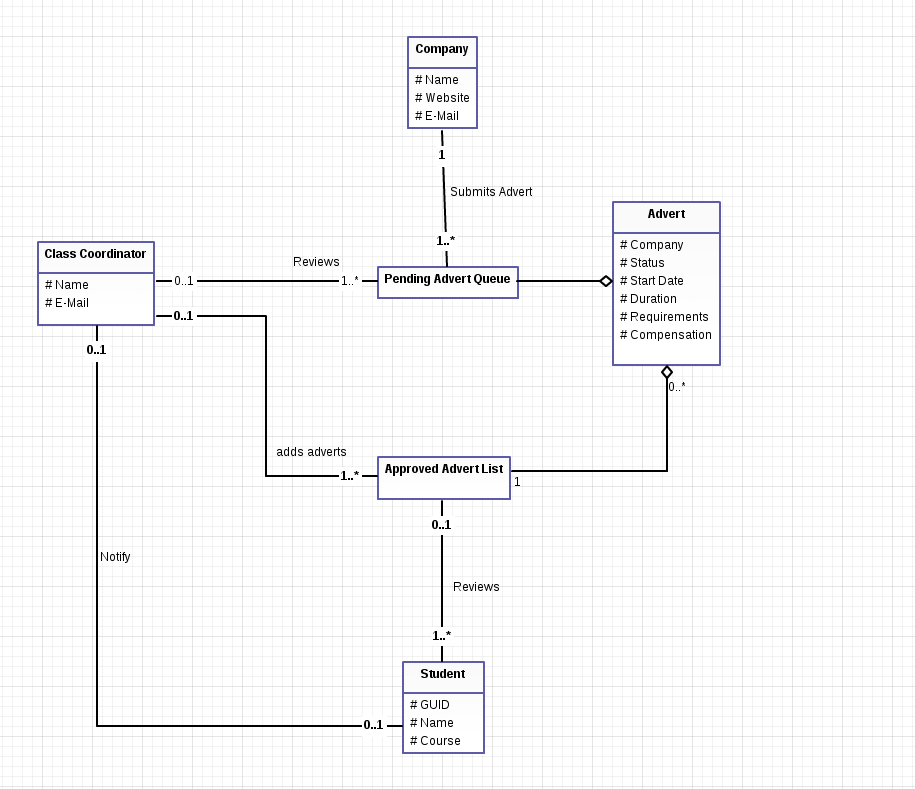
\includegraphics
[scale=0.7]
{img/UML.png}
\caption{Domain model}
\label{fig1:domain model}
\end{center}
\end{figure}

%%%%%%%%%%%%%%%%%%%%%%%%%%%%%%%%%%%%%%%%%%%%%%%
%%%%%%%%%%%%%%%%%%%%%%%%%%%%%%%

\section{Use Case Descriptions}

This section describes the required functionality for the internship management system as four groups of related
use cases. The core use cases for the system are:\\

\textbf{Submission of internship advert by Company (Section 4.1):}
\begin{itemize}
\item Submit internship advert
\item Edit advert
\end{itemize}

\textbf{Review and approval of internship adverts by Course Co-ordinator (Section 4.2):}
\begin{itemize}
\item Review internship adverts
\item Approve internship advert
\end{itemize}

\textbf{Review of adverts by Student (Section 4.3):}
\begin{itemize}
\item View internship adverts
\item Apply for internship
\end{itemize}

\textbf{Notification of successful internship placement by student (Section 4.4):}
\begin{itemize}
\item Notify Course Co-ordinator of successful placement
\item Remove internship advert
\end{itemize}

\textbf{Common utility services (Section 4.5):}
\begin{itemize}
\item Login
\item Logout
\end{itemize}

\subsection{Submission of internship advert by Company}
\begin{figure}[h]
\begin{center}
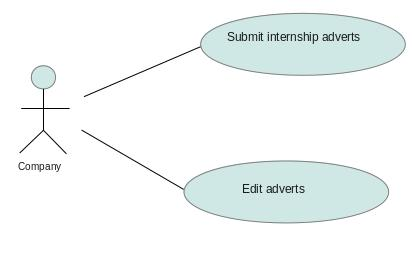
\includegraphics
[scale=0.7]
{img/Company.jpeg}
\caption{Use Case Diagram 4.1}
\label{fig2:Use Case Diagram4.1}
\end{center}
\end{figure}

\begin{UseCaseTemplate}
\UseCaseLabel{Submit internship advert}
\UseCaseDescription{A company should login and post internship adverts to the system,
confirm it and logout.}
\UseCaseRationale{During the client interview we were given the requirement that a company must be able to submit internship adverts to the system in order for the students to view and apply for the placement.}
\UseCasePriority{Must have}
\UseCaseStatus{Not implemented}
\UseCaseActors{Company}
\UseCaseIncludes{Login, Logout}
\UseCaseConditions{Post: The advert is stored in the system, pending approval by the CC.}
\UseCaseNonFunctionalRequirements{Security}
\UseCaseScenarios{IBM are wanting to submit an internship advert to the system. They log in to the system using their designated username IBM, fill out the submission form, confirm their submission and submit it to the system to eventually be approved by Timothy Storer, the current CC. IBM then log out of the system.}
\UseCaseRisks{}
\end{UseCaseTemplate}

\begin{UseCaseTemplate}
\UseCaseLabel{Edit internship advert}
\UseCaseDescription{A company must login, make changes to their advert where necessary,
confirm changes and then logout.}
\UseCaseRationale{During the stakeholder panel meeting the need for companies to be able to edit pending approval adverts was clarified to be a requirement.}
\UseCasePriority{Must Have}
\UseCaseStatus{Not implemented}
\UseCaseActors{Company}
\UseCaseIncludes{Login, Logout}
\UseCaseConditions{Pre: Company's advert must currently be pending approval by the CC.}
\UseCaseNonFunctionalRequirements{Data consistency}
\UseCaseScenarios{IBM realise that the advert they have previously submitted contains the wrong starting date. They log in to the system, select the relevant advert and section they want to edit and correct the starting date. They confirm their changes and then log out.}
\UseCaseRisks{During client interview we were told that this probably wouldn't be needed, yet during the stakeholder panel meeting it was made clear that it was a valid requirement.}
\end{UseCaseTemplate}

\subsection{Review and approval of internship adverts by Course Co-ordinator}

\begin{figure}[h]
\begin{center}
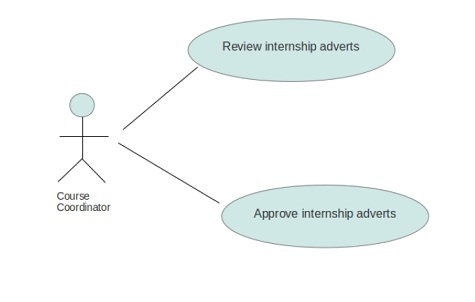
\includegraphics
[scale=0.7]
{img/CourseCoordinator.jpg}
\caption{Use Case Diagram 4.2}
\label{fig2:Use Case Diagram4.2}
\end{center}
\end{figure}

\begin{UseCaseTemplate}
\UseCaseLabel{Review internship adverts}
\UseCaseDescription{CC must login, read through new/edited adverts posted
and decide if they are suitable for the students.}
\UseCaseRationale{During the client interview we verified that it was essential for the CC to have the ability to review adverts.}
\UseCasePriority{Must have}
\UseCaseStatus{Not implemented}
\UseCaseActors{Course Co-ordinator}
\UseCaseIncludes{Login, Logout}
\UseCaseConditions{Pre: Must have advert(s) pending approval on system.}
\UseCaseNonFunctionalRequirements{Data consistency}
\UseCaseScenarios{Timothy Storer, the current CC, logs in to the system with his GUID and views all pending adverts submitted to the system and decides whether or not each internship is suitable for student review.}
\UseCaseRisks{}
\end{UseCaseTemplate}
\begin{UseCaseTemplate}

\UseCaseLabel{Approve internship advert}
\UseCaseDescription{Course Coordinator must login. After reviewing the adverts and deciding
they are suitable, the adverts are made available to the students.}
\UseCaseRationale{During the client interview we verified that it was essential for the CC to have the ability to approve adverts.}
\UseCasePriority{Must have}
\UseCaseStatus{Not implemented}
\UseCaseActors{Course coordinator}
\UseCaseIncludes{Login, Logout}
\UseCaseConditions{Pre: Must have advert(s) pending approval on system. Pre: adverts reviewed by course coordinator}
\UseCaseNonFunctionalRequirements{Data consistency}
\UseCaseScenarios{After having reviewed an internship advert from IBM, Timothy Storer, the current CC, decides that the advert is suitable. He specifies what degree structure (CS/SE/ESE) it's suitable for and approves the advert for later student review.}
\UseCaseRisks{}
\end{UseCaseTemplate}

\subsection{Review of Advertisement by Student}

\begin{figure}[h]
\begin{center}
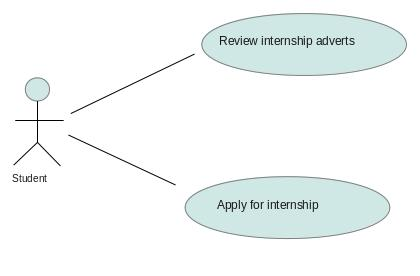
\includegraphics
[scale=0.7]
{img/Student.jpeg}
\caption{Use Case Diagram 4.3}
\label{fig2:Use Case Diagram4.3}
\end{center}
\end{figure}

\begin{UseCaseTemplate}
\UseCaseLabel{View internship adverts list}
\UseCaseDescription{List of adverts is displayed on screen and users scrolls through and can read detailed information about the internship.}
\UseCaseRationale{User needs to be able to see the adverts in order to apply.}
\UseCasePriority{Must Have}
\UseCaseStatus{Not Implemented}
\UseCaseActors{Student}
\UseCaseIncludes{Login, Logout, Apply for internship}
\UseCaseConditions{Pre: adverts have been approved by the CC.}
\UseCaseNonFunctionalRequirements{}
\UseCaseScenarios{}
\UseCaseRisks{}
\end{UseCaseTemplate}

\begin{UseCaseTemplate}
\UseCaseLabel{Apply for internship}
\UseCaseDescription{User selects an advert to apply for and will then have to email the company or will be directed to the company website to apply}
\UseCaseRationale{Student should be redirected to the company URL or email in order to apply for the internship placement.}
\UseCasePriority{Must Have}
\UseCaseStatus{Not Implemented}
\UseCaseActors{Student}
\UseCaseIncludes{Login,Logout}
\UseCaseConditions{}
\UseCaseNonFunctionalRequirements{}
\UseCaseScenarios{The student will select the apply option within the system. The student will then be redirected to the company website in order to fill out the application for the internship.}
\UseCaseRisks{The email/website may be incorrect so student may not be able to apply.}
\end{UseCaseTemplate}

\subsection{Notification of successful selection for an internship by an SE/ESE student}

\begin{figure}[h]
\begin{center}
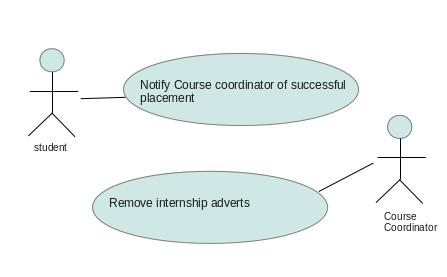
\includegraphics
[scale=0.7]
{img/Section4.jpeg}
\caption{Use Case Diagram 4.4}
\label{fig2:Use Case Diagram4.4}
\end{center}
\end{figure}

\begin{UseCaseTemplate}
\UseCaseLabel{Notify course coordinator of successful placement}
\UseCaseDescription{Let course coordinator know a Placement position has been filled.}
\UseCaseRationale{A student should let the Course Coordinator know that they were successful
with their application for a specified placement position so that the CC can go on and remove
the advert from the System.}
\UseCasePriority{Must have.}
\UseCaseStatus{Not Implemented}
\UseCaseActors{Student}
\UseCaseIncludes{Login,Logout}
\UseCaseConditions{Pre: The advert for the placement position that was taken must be still
visible on the system. Post: Course Coordinator is notified.}
\UseCaseNonFunctionalRequirements{}
\UseCaseScenarios{A student has been successful with a placement with one of the adverts on the system. The student will notfiy the Course coordinator of there successful placement within the system and the course coordinator will receive an email.}
\UseCaseRisks{}
\end{UseCaseTemplate}

\begin{UseCaseTemplate}
\UseCaseLabel{remove internship adverts}
\UseCaseDescription{Course Coordinator logins in to system. If advert is passed deadline or no
longer suitable or available, the advert will be taken off the system and then log out.}
\UseCaseRationale{A member of the school of computing science (course coordinator) is
responsible for taking adverts down so as to avoid students applying for internships that are no
longer available or suitable.}
\UseCasePriority{Must have}
\UseCaseStatus{Not implemented}
\UseCaseActors{Course coordinator}
\UseCaseIncludes{Login,Logout}
\UseCaseConditions{Pre: Course Coordinator has recieved a notification to say the placement has been filled. Post: Advert no longer available on the system.}
\UseCaseNonFunctionalRequirements{}
\UseCaseScenarios{The course coordinator has recieved a notification of a successful placement and logs into the system. The course coordinator then removes the internship advert from the system, so that it is no longer available to the students.}
\UseCaseRisks{Course Coordinator might remove the wrong advert.}
\end{UseCaseTemplate}

\subsection{Common utility services}

\begin{UseCaseTemplate}
\UseCaseLabel{Login}
\UseCaseDescription{A user should enter their login id and a password to allow them to access
the system. }
\UseCaseRationale{A user must be able to login, providing different levels of access to the system.}
\UseCasePriority{Must have}
\UseCaseStatus{Not implemented}
\UseCaseActors{Company, Students, Course Coordinator}
\UseCaseIncludes{}
\UseCaseConditions{}
\UseCaseNonFunctionalRequirements{}
\UseCaseScenarios{}
\UseCaseRisks{}
\end{UseCaseTemplate}

\begin{UseCaseTemplate}
\UseCaseLabel{Logout}
\UseCaseDescription{The logout use cases changes a users account to logged out, requiring
them to have to log back in to the system. Logout is either invoked by the user or by the internal
inactivity timer actor.}
\UseCaseRationale{The logout case will allow a user to leave the system to prevent
unauthorised access from an unattended terminal.}
\UseCasePriority{Must Have}
\UseCaseStatus{Not implemented}
\UseCaseActors{Company, Students, Course Coordinator}
\UseCaseIncludes{}
\UseCaseConditions{Pre: User must be logged in to the system.}
\UseCaseNonFunctionalRequirements{}
\UseCaseScenarios{}
\UseCaseRisks{}
\end{UseCaseTemplate}

%%%%%%%%%%%%%%%%%%%%%%%%%%%%%%%%%%%%%%%%%%%%%%%
%%%%%%%%%%%%%%%%%%%%%%%%%%%%%%%
\section{Non Functional Requirements}

\begin{itemize}
\item User Concurrency: The system should be available to all Students of the School of Computing Science and a large number of users might want to use the system at the same time so the System should be able to handle a large number of users at once.
\item Data Consistency: The system must maintain data accuracy and integrity throughout the sytem's use, to ensure that each user observes a consistent view of the data despite any changes made by other users.
\item Security: Students should be able to log in with their GUIDs and passowrds which would be the same used for other University of Glasgow websites such as Moodle and MyCampus. Employers who wish to use the system to post placement adverts will need to be provided with new usernames and passwords in order to use the system.
\item Number of Adverts: The system must be able to handle an unlimited number of adverts. Any number of companies might offer placement opportunities for students each year therefore the number of adverts that can be posted on the system must not be limited.
\end{itemize}

%%%%%%%%%%%%%%%%%%%%%%%%%%%%%%%%%%%%%%%%%%%%%%%
%%%%%%%%%%%%%%%%%%%%%%%%%%%%%%%
\section{Summary}

A company should upload their adverts to the system. The course coordinator will review
all adverts posted to the system and determine whether or not they are appropriate for the
students. If appropriate, the CC makes the advert available for the students to view. If a student
wants to apply for an advert, they will email the company or apply through their website. If
a student successfully secures a placement, they must notify the course coordinator. If all
placements have been filled, the CC can take the adverts off the system.

%%%%%%%%%%%%%%%%%%%%%%%%%%%%%%%%%%%%%%%%%%%%%%%
%%%%%%%%%%%%%%%%%%%%%%%%%%%%%%%
\appendix

\section{Glossary}
CC - Course Co-ordinator
PSD - Professional Software Development

\section{Stakeholder Interview Documentation}

Key points we got from our interview with the client are:

\begin{itemize}
\item The company does not directly interact with the system.
\item The Course Coordinator will review adverts sent via email and if they are suitable, would
then be posted on the system.
\item When applying for internships, students will be redirected to the company website or given
an email address in order to send in their CV.
\item Students will be able to flag inappropriate adverts to the CC.
\item Students will notify the CC of a successful placement via email.
\item The Company must also verify a successful placement to avoid students abusing the
system.
\item Once a student has accepted a placement, the advert is taken off the system.
\end{itemize}

\section{Stakeholder Panel Documentation}

Originally, we were informed that the company would not interact with the system, all adverts
would be submitted via email to the course coordinator. However, at the stakeholder meeting
it was clarified that the company would interact with the system. The company will be given a
username and password and will be able to post their adverts directly to the system. They will
have a to fill out a standard form with all the relevant information before submitting the advert.
The course coordinator will then review it to determine whether or not it is relevant for the
students. If so, the adverts is made available to the students.
%%%%%%%%%%%%%%%%%%%%%%%%%%%%%%%%%%%%%%%%%%%%%%%
%%%%%%%%%%%%%%%%%%%%%%%%%%%%%%%
\end{document}
%%%%%%%%%%%%%%%%%%%%%%%%%%%%%%%%%%%%%%%%%%%%%%%
%%%%%%%%%%%%%%%%%%%%%%%%%%%%%%%

